\chapter{Tau Pair Polarisation Correlation}
\label{chap:Tau2Mini}

\chapterquote{Where can I find a man who has forgotten words so I can have a word with him?}%
{Zhuang Zi, 369 BC $-$ 286 BC}%: Blackwood's Magazine May 1830



%\section{Tau pair polarisation correlations as a signature of Higgs boson decay}
%\label{sec:tauHZ}

This chapter follows the theoretical discussion in \Section{sec:theoryTauPair} on using the correlation between the polarisations of the tau pair from a boson decay as a signature to differentiate the Higgs boson from the \PZ boson.

A  spin-0 scalar Higgs boson can decay to \TauTauSub{L}{L} or \TauTauSub{R}{R}, whereas the  spin-1 \PZ  boson can decay to \TauTauSub{L}{R} or \TauTauSub{R}{L}, where L, R denote the tau lepton helicities. Therefore, by studying the tau pair polarisation correlation from a boson decay, one can determine statistically if the parent boson is a  scalar or a vector.

Here a proof-of-principle analysis  is performed to reconstruct the polarisation correlation of the tau pairs in the \ZToTauTau process, where both \tauToPionBoth. \tauToPionBoth decay mode is selected using the tau decay mode classifier developed in \Chapter{chap:Tau}, which utilises the photon reconstruction in a highly granular calorimeter developed in \Chapter{chap:Photon}. The charged pion decay mode is chosen because the correlation between $E_{\Ppiplus} / E_{\APtauon}$ and $E_{\Ppiminus} / E_{\Ptauon}$ is very different if the parent boson is a \PZ or a \PHiggs boson, as suggested in \Figure{fig:theoryTauPairCorrelation}.


The analysis starts with the event generation and simulation, followed by identifying the tau decay products in the events. Afterwards, the tau decay mode classification is used to identify \tauToPionBoth decays. Lastly the tau pair polarisation correlation is presented and compared to  the tau pair polarisation correlation obtained with generator-level Monte Carlo particles. \FIGURE{fig:TauNTAflow} shows main steps in this proof-of-principle demonstration of the tau pair polarisation correlations using  \eeZZQQ events, where both \tauToPionBoth.



\begin{figure}[htbp]
\centering % \begin{center}/\end{center} takes some additional vertical space
  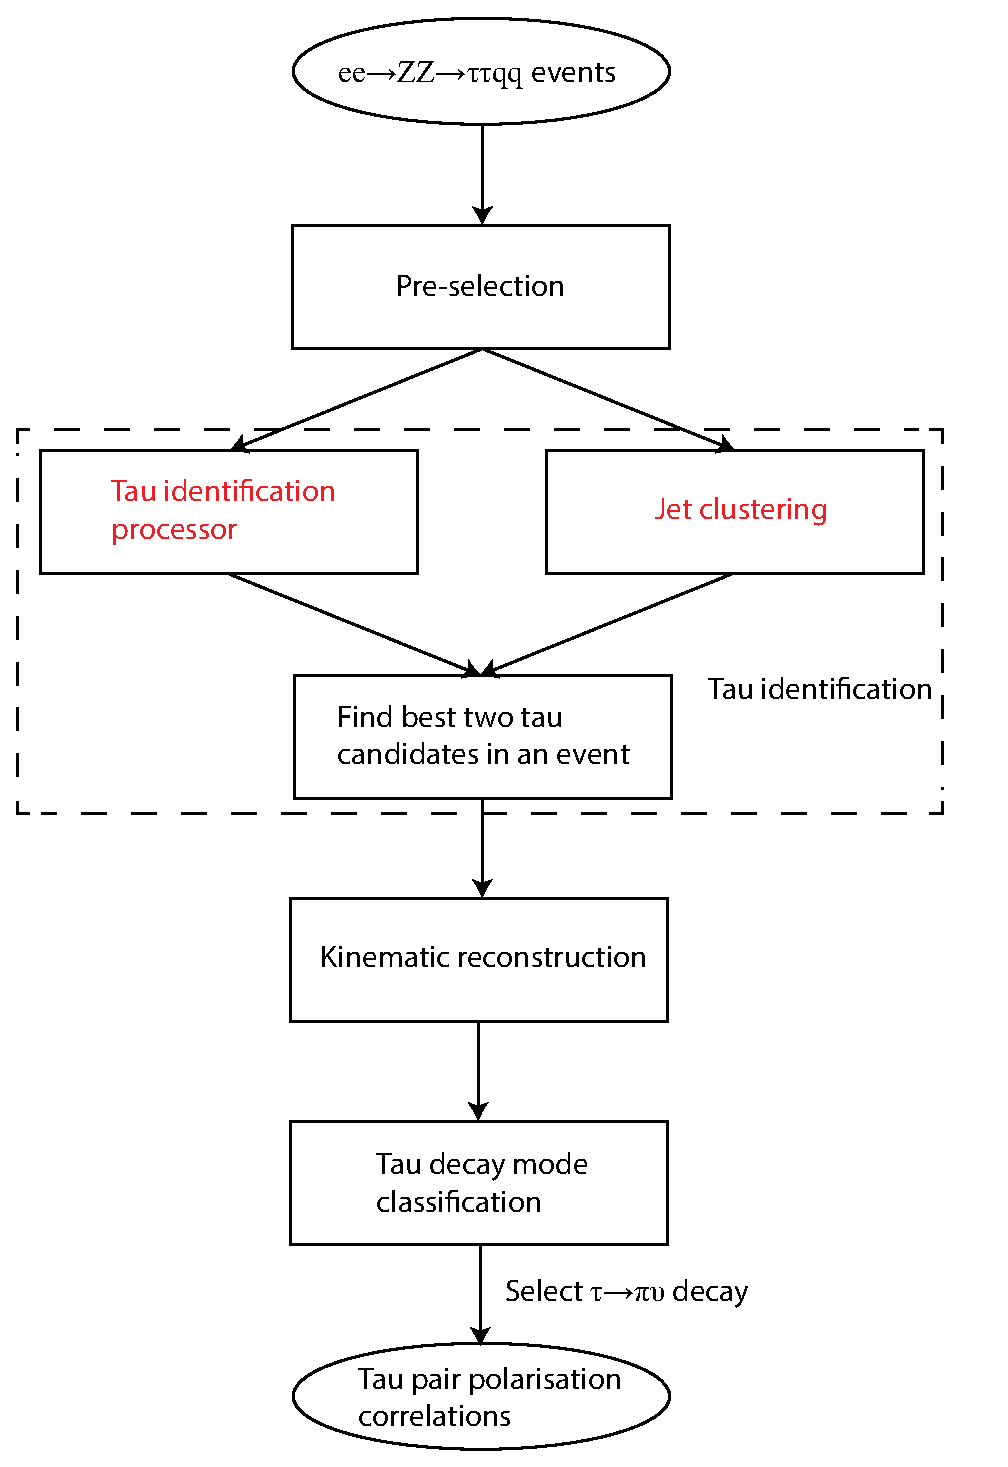
\includegraphics[width=0.75\textwidth]{tau/NoTimeAnalysis/tauNTAflow2}
  \caption{Main steps in the proof-of-principle demonstration of the tau pair polarisation correlations.}
  \label{fig:TauNTAflow}
\end{figure}



%For many theories beyond the Standard Model, a common feature is that the coupling of the Higgs particle to leptons increases with the increase of the lepton mass \cite{Duperrin:2008in}.  In these BSM theories, unlike vector bosons coupling to all flavours of leptons equally, the \HigssTauTau coupling would dominate the Higgs coupling to leptons. Therefore, if an experiment observes the breaking of the lepton universality by favouring \TauTau events, it could indicate the existence of a scalar Higgs. When such a universality breaking is observed, a helicity correlation test can be used to show that the \TauTau pair is from a scalar boson or a vector boson. In particular, the polarisation correlations of tau leptons are different for \HiggsToTauTau and \ZToTauTau, as scalar Higgs decays to \TauTauSub{L}{L} or \TauTauSub{R}{R} and \PZ decays to \TauTauSub{L}{R} or \TauTauSub{R}{L}, where L, R denotes the tau lepton helicities.


%Tau pair polarisation correlations can be studied using various tay decay modes. Here \Reference{Bullock:1991my} is followed and the \tauToPion decay mode is used as the example. The Higgs and \PZ boson decay to a  tau pair, where both tau leptons subsequently decay   via  \tauToPion, can be represented as:



%Many BSM theories predict the \HigssTauTau coupling would dominate the Higgs boson to leptons couplings  \cite{Duperrin:2008in}. Therefore, if an experiment observes an excess of tau pair decay events, it could be an indication of the Higgs boson. Here, this section follows


%Comparing \HiggsToTauTau  and \ZToTauTau, the difference in the spin of the bosons reflects in the different polarisation correlation of the tau pair. By extracting the polarisation correlations of the tau pair, the parent boson can be identified.

%The subsequent sections discuss the ability to reconstruct the polarisation correlation of the tau pair with \ZToTauTau channel, where both \tauToPion. The analysis starts with the event pre-selection, followed by identifying the tau decay products in the events. Afterwards, the tau decay mode classification is used to identify \tauToPion decays. Lastly the tau pair polarisation correlation is presented and compared to the correlation distribution obtained with Monte Carlo simulation.

\section{Event generation and simulation}

For this proof-of-principle study, \eeZZQQ events were generated at a centre-of-mass energy of 350\,GeV, using \WHIZARD \cite{whizard} generator without ISR. \TAUOLA \cite{Jadach:1993hs} was used to describe the tau lepton decay with correct spin correlations of the tau decay products. Beam effects, such as the initial state radiation and the beam induced background, were not included. The \eeZZQQ events were simulated using the \ILD detector model as described in \Chapter{chap:Reconstruction}.


%\subsection{Analysis strategy overview}

%The goal of the analysis is to obtain the distributions of  $E_{\Ppiplus} / E_{\APtauon}$ and $E_{\Ppiminus} / E_{\Ptauon}$, using the \tauToPionBoth decays of both taus in \eeZZQQ events. Because the energy of the taus can be obtained in the \ZToTauTau rest frame, and events were generated in the \PZ rest frame in the tau decay mode classifier study, the tau decay products were boosted into the \PZ rest frame.  For  the tau decay products, the charged pion decay mode is selected using the tau decay mode classifier. Identifying the tau decay products in \eeZZQQ events is challenging as a low multiplicity quark-jet could be topologically similar  to a tau-jet.
\section{Event reconstruction}


Events were reconstructed with  \ilcsoft version v01-17-07 \cite{Gaede:82475} and \pandora version 3 \cite{Marshall:2015rfa}, using the photon reconstruction algorithms described in \Chapter{chap:Photon}. \FIGURE{fig:TauNTAevtDsp} shows an event display of a \eeZZQQ event. The two brown cones indicate the tau decay products found by the tau identification processor. The four blue cones indicate the four jets found by the jet clustering algorithm.


%Hence the two approaches are combined to find the decay products from two tau leptons.
% The best tau decay products should result in a well reconstructed \ZToqq.

%For a low multiplicity tau-jet, it is beneficial to use a dedicated tau decay product identification processor. For a high multiplicity tau-jet, the jet clustering algorithm may be more suitable to find tau decay products.


\begin{figure}[htbp]
\centering % \begin{center}/\end{center} takes some additional vertical space
  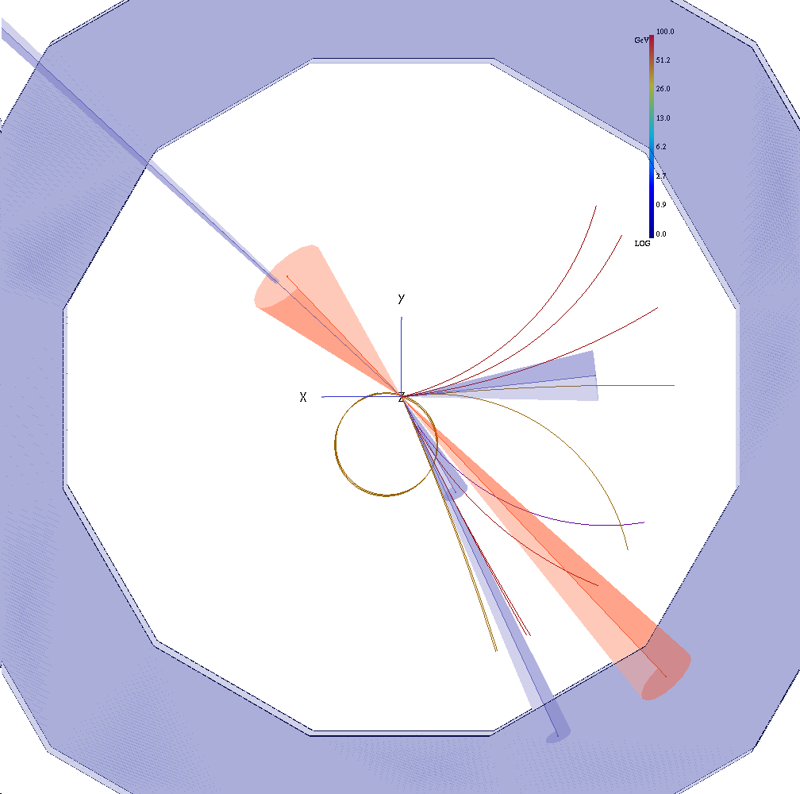
\includegraphics[width=0.65\textwidth]{tau/NoTimeAnalysis/EvtDsp}
  \caption{An event display of a \eeZZQQ event. The two brown cones indicate the tau decay products found by the tau identification processor. The four blue cones indicate the four jets found by the jet clustering algorithm. The blue outer region shows the \HCAL ring.}
  \label{fig:TauNTAevtDsp}
\end{figure}


Seven tau decay modes defined in \Section{sec:tauDecayModes} were considered in this analysis: \tauToElectron; \tauToMuon; \tauToPion; \tauToRho; \tauToAiPhoton; \tauToAiPion; and \tauToThreePion.


\section{Pre-selection}

Two pre-selection cuts defined in \Section{sec:tauPreSel} are used: the tau decay products with photon conversion to electron pairs in the tracking detector are not considered; and tau decays with the generated polar angle of the tau lepton in the region $0.6 < \absOf{\theta_{\Ptau}^{MC}} < 0.9$\,rad are not considered.


%Since this study is focused on photon reconstruction in the \ECAL to classify tau decay modes, the tau decays with photon converting to electron pairs in the tracking detector are not considered.

%The focus of the study is on higher energy tau decays. Tau decays with the total visible energy (i.e. not accounting for neutrinos) of tau decay products, $E_{vis}^{MC}$, less than 5\,GeV are not considered.

\section{Tau identification}
\label{sec:tauHZfindTau}

The \eeZZQQ final state contains two tau leptons and two quark jets. Identifying the tau decay products in \eeZZQQ events is challenging as a low multiplicity quark-jet could be topologically similar  to a tau hadronic decay. Hence the tau decay product identification processor and the jet clustering algorithm are both used to find tau decay products. In the event shown in \Figure{fig:TauNTAevtDsp}, particles associated with the tau decay products found by the tau identification processor are different to the particles associated with jets found by the jet clustering algorithm.

%\FIGURE{fig:TauNTAevtDsp} shows an event display of a \eeZZQQ event. The two brown cones indicate the tau decay products found by the tau identification processor. The four blue cones indicate the four jets found by the jet clustering algorithm.
%The blue outer region shows the \HCAL ring. In this particular example, particles associated with the tau decay products found by the tau identification processor are different to the particles associated with jets found by the jet clustering algorithm.

%Therefore, tau decay products can either be found by direct tau lepton decay products searching with a tau finder processor, or by using jet algorithms to find tau decay products as jets. When a tau lepton decays to a few particles, such as the leptonic tau decay final states, the direct tau searching method is favoured. When a tau lepton decays hadronically, resulting in multiple charged and neutral particles, the jet cluster method is suitable to find tau decay methods. Hence, two approaches are combined to find the two tau leptons decay products.





%The studied process  is \HepProcess{\Pep \Pem \to \PZ \PZ}, where one \PZ boson decays hadronically and the other \PZ boson decays to a tau lepton pair. The samples were generated at a centre-of-mass energy of 350\,GeV without \ISR contribution for this proof-of-principle study.

%The same seven tau decay modes defined in the previous analysis in \Section{sec:tauDecayModes} are studied. The constraints on the simulated events are the same as those   in the previous analysis in \Section{sec:tauSim}, except that the constraint on the total energy of non-neutrino decay products is not applied. A considerable fraction of \ZToTauTau events, where \tauToPion, have two low-energy charged pions. Therefore, the constraint on the total energy of non-neutrino decay products would distort the energy distribution of the charged pions, thus affecting the tau pair polarisation correlation extration.

 %The \tauToPion decay mode is selected for the proof-of-principle analysis of \PHiggs/\PZ separation with tau pair decay channel.

%\subsection{Find tau decay products}

%If a tau lepton decays into a few particles, then the direct tau searching would work better. If a tau lepton decays into many particles, finding tau decay products as jets has a better performance, as jet clustering works better with more particles.

\subsection{Tau identification processor}
\label{sec:TauMiniTauIdentifier}

The \BonoTauFinder processor is a modified version of the tau decay product identification software used in the double Higgs analysis in \Section{sec:doubleHiggsBonoTauFinder}. The processor identifies high transverse momentum (\pT) particles as tau seeds. Particles are iteratively added to a cone in the order of the ascending opening angle to the seed. The cone is called search cone, which contains potential tau decay products. After each particle addition, the temporary search cone is then considered as a temporary  tau candidate and tested for isolation and consistency  with a tau hadronic decay signature. The number of charged particles in the temporary tau candidate, $N_{X^+}$, should be one or three. The invariant mass of the temporary tau candidate, $m_{c}$, should be less than 3\,GeV. The temporary tau candidate also needs to pass the isolation condition to be identified as a tau candidate, which requires the opening angle between the temporary search cone  and the $2^{nd}$ closest charged particle, $\theta^{c}_{X'^+}$, is larger than 0.6\,rad.

The iterative particle addition procedure stops when the cone opening angle, $\theta_S$, is larger than $\cos^{-1}(0.99)$. If multiple temporary tau candidates of the same tau seed pass the isolation condition, the one with the smallest opening angle is chosen to form the final tau candidate. \TABLE{tab:tauBonoTauFinderProcessor} lists the parameters  of the  \BonoTauFinder processor.

%The parameter \pT is the transverse momentum. The parameter $\theta_S$ is the maximum opening angle of the search cone in rad. The parameter $ N_{X^+}$ is the number of charged particles in the search cone. The parameter $m_{c}$ is the invariant mass of all particles in the search cone. The parameter $\theta^{c}{X'^+}$ is the opening angle between the search cone  and the $2^{nd}$ closest charged particle.

%Variables are defined in the same way as those in previous sections In addition, $\theta_S$ is the opening angle of the search cone in rad; $cone1$ and $cone2$ are defined as a cone around the tau seed of an opening angle of $\cos^{-1}(0.95)$, and $\cos^{-1}(0.99)$ respectively.


%Particles with energies less than 0.5\,GeV are not considered, to reduce the fake rate from the potential beam background.

%There are multiple isolation conditions for tau 1-prong decay and 3-prong decay, reflecting different topologies of tau decay final states. The isolation criterion typically demand few particles around the search cone and the total \pT in the search cone to be greater than a threshold.



%The idea is to find tau decay products consistent with tau decay topologies, and to require the tau  decay products to be isolated from the rest of the particles.

%Parameters chosen are set to find as many tau candidates as possible.

%The filtering of the candidates is via kinematic constraints.

%\TABLE{tab:tauBonoTauFinderProcessor} lists all the cuts used in the \BonoTauFinder. Particles with transverse momentum (\pT) less than 0.5\,GeV are not considered. A seed particle is chosen and a search cone is formed around the seed, which requires one or three tracks with the invariant mass  of all particles inside the search cone ($m_{c}$) less than 3\,GeV. Particles are iteratively added to the search cone with a gradually widening opening angle of the search cone. The maximum search cone opening angle ($\theta_S$) is $\cos^{-1}(0.99)$. The isolation criteria states that the opening angle between the search cone  and the $2^{nd}$ closest charged particle ($\theta_{c-2^{nd}X^+}$) is larger than 0.6\,rad. If the criteria is satisfied,  particles associated with the search cone  is identified are the decay products of one tau lepton.

\begin{table}[!htbp]
\begin{tabular}{lr}
\hline
\hline
Modified \BonoTauFinder  & Selection \\
\hline
Veto low \pT &  $\pT < 0.5$\,GeV\\
Seed particle & $\pT > 1$\,GeV \\
Maximum search cone opening angle  & $\theta_S \leqslant \cos^{-1}(0.99)$\\
Tau candidate rejection & $N_{X^+} \neq$ 1 or 3; $m_{c} > 3$\,GeV   \\
Isolation & $\theta^{c}_{X'^+} > 0.6$\,rad\\
\hline
\hline
\end{tabular}
\caption
{Optimised parameters of the modified \BonoTauFinder.}
\label{tab:tauBonoTauFinderProcessor}
\end{table}

The event is discarded if the \BonoTauFinder processor finds fewer than two tau candidates. If more than two tau candidates are found, the best two are selected by choosing the tau candidates that gives the smallest value of the $\chi^2$ function, resulting in well reconstructed \ZToqq decays:
\begin{equation}
\chi^2 = {\parenths{m_{\Pquark\Pquark} - m_{\PZ}}^2}+ {\parenths{E_{\Pquark\Pquark} - \frac{\sqrtS}{2}}^2},
\label{eq:tauMinimiser}
\end{equation}
where \sqrtS is the centre-of-mass energy;   variable $m_{\PZ}$ is the mass of \PZ boson from reference \cite{Agashe:2014kda};  $m_{\Pquark\Pquark}$ is the invariant mass of particles that do not belong to the two tau candidates; and  $E_{\Pquark\Pquark}$ is  the total energy of particles that do not belong to the two tau candidates. This function is considered for all pairs of tau candidates.  In the generated \eeZZQQ events, the energy of each \PZ boson is half of the centre-of-mass energy. The invariant mass of two quarks from the \PZ decay should be close to \PZ mass.






%the reconstructed mass resolution  and energy resolution of the \ZToqq, respectively;  the variables $m_{\Pquark\Pquark}$ and  $E_{\Pquark\Pquark}$ are obtained from the recoil momenta against two tau candidates, assuming that the collision occurs at \sqrtS. The  $m_{\Pquark\Pquark}$ is defined as the invariant mass of the recoil momenta, and  the $E_{\Pquark\Pquark}$ is defined as the energy of the recoil momenta.; and the minimisation is iterated over all tau candidates.

\subsection{Jet clustering}

%Tau hadronically decay products can be also identified as a small jet.

The Durham algorithm  (see \Section{sec:pandoraJetDurham}) was run in the exclusive mode to force the reconstructed particles in \eeZZQQ events into exactly four jets. The two tau candidate jets are identified by selecting two jets that gives the smallest value of the $\chi^2$ function in \Equation{eq:tauMinimiser}. Here $m_{\Pquark\Pquark}$ is the invariant mass of particles that are not in the two tau candidates jets and $E_{\Pquark\Pquark}$ is  the total energy of particles that are not in the two tau candidates jets. Other variables are defined in the same way as in \Section{sec:TauMiniTauIdentifier}.



%find four jets for \eeZZQQ events.

%Two jets correspond to two quark jets and the other two jets correspond to two tau lepton decay products.
\begin{comment}
\subsubsection{Selecting best tau candidates for each tau finding method}

The direct tau searching method may find more than two tau  candidates, where each tau candidate corresponds to one tau lepton decay products. To identified the best two tau candidates, kinematic constraints are used.  For example, in  \HepProcess{\Pep \Pem \to \PZ \PZ} events, the energy of the \PZ boson is half of the centre-of-mass energy. The invariant mass of two quarks from \PZ should be close to \PZ mass. Therefore, the $\chi^2$ minimisation function utilising kinematic constraints is:
\begin{equation}
\chi^2 = \frac{\parenths{m_{\Pquark\Pquark} - m_{\PZ}}^2}{\sigma_{m_{\Pquark\Pquark}}^2} + \frac{\parenths{E_{\Pquark\Pquark} - \frac{\sqrtS}{2}}^2}{\sigma_{E_{\Pquark\Pquark}}^2},
\label{eq:tauMinimiser}
\end{equation}
where \sqrtS is the centre-of-mass energy; the variable $m_{\PZ}$ is the mass of \PZ boson from reference \cite{Agashe:2014kda}; the variables $\sigma_{m_{\Pquark\Pquark}}$ and $\sigma_{E_{\Pquark\Pquark}}$ are the reconstructed mass resolution  and energy resolution of the \ZToqq, respectively;  the variables $m_{\Pquark\Pquark}$ and  $E_{\Pquark\Pquark}$ are obtained from the recoil momenta against two tau candidates, assuming that the collision occurs at \sqrtS. The  $m_{\Pquark\Pquark}$ is defined as the invariant mass of the recoil momenta, and  the $E_{\Pquark\Pquark}$ is defined as the energy of the recoil momenta.; and the minimisation is iterated over all tau candidates.

This minimisation produces two best tau candidates for the direct tau searching method. For the jet clustering method, to find the two jets corresponding to two tau lepton decay, the same $\chi^2$ minimisation function is used.  The variables $m_{\Pquark\Pquark}$ and  $E_{\Pquark\Pquark}$ are defined as the total invariant mass and energy of two non-tau-candidate jets, respectively. All other variables in the minimisation function are defined in the same way. After applying the minimisation function, two jets will be identified as the best two tau candidates from the jet clustering method.


%Each of the above two methods produces potentially more than two tau candidates. For example, the direct tau searching method may find many tau candidates


Each tau candidate corresponds to one tau lepton decay products from the direct tau searching method, or one jet from the jet clustering method. To identified the best two tau candidates within a method, kinematic constraints are used.  For example, in  \HepProcess{\Pep \Pem \to \PZ \PZ} events, the energy of the \PZ boson is half of the centre-of-mass energy. The invariant mass of two quarks from \PZ should be close to \PZ mass. Therefore, the $\chi^2$ minimisation function utilising kinematic constraints is:
\begin{equation}
\chi^2 = \frac{\parenths{m_{\Pquark\Pquark} - m_{\PZ}}^2}{\sigma_{m_{\Pquark\Pquark}}^2} + \frac{\parenths{E_{\Pquark\Pquark} - \frac{\sqrtS}{2}}^2}{\sigma_{E_{\Pquark\Pquark}}^2},
\label{eq:tauMinimiser}
\end{equation}
where \sqrtS is the centre-of-mass energy; the variable $m_{\PZ}$ is the mass of \PZ boson from reference \cite{Agashe:2014kda}; the variables $\sigma_{m_{\Pquark\Pquark}}$ and $\sigma_{E_{\Pquark\Pquark}}$ are the reconstructed mass resolution  and energy resolution of the \ZToqq, respectively;  the variables $m_{\Pquark\Pquark}$ and  $E_{\Pquark\Pquark}$ are defined differently for the direct tau searching and the jet clustering methods; and the minimisation is iterated over all tau candidates  from direct tau searching method or over all jets from jet clustering method.

For the direct tau searching method, $m_{\Pquark\Pquark}$ and  $E_{\Pquark\Pquark}$ are obtained from the recoil momenta against two tau candidates, assuming that the collision occurs at \sqrtS. The  $m_{\Pquark\Pquark}$ is defined as the invariant mass of the recoil momenta, and  the $E_{\Pquark\Pquark}$ is defined as the energy of the recoil momenta. For the jet clustering method,  $m_{\Pquark\Pquark}$ and  $E_{\Pquark\Pquark}$ are defined as the total invariant mass and energy of two non-tau-candidate jets, respectively.

The $\chi^2$ minimisation function is repeated for the direct tau searching method and the jet clustering method. For each method, the minimisation produces a best pair of  tau candidates with the smallest $\chi^2$.
\end{comment}

\subsection{Selecting best tau candidates in an event}


If both \BonoTauFinder processor and the jet clustering method find two tau candidates, the best pair of tau  candidates   should result in well reconstructed \ZToqq decays, defined by:
\begin{equation}
\absOf{m_{\Pquark\Pquark} - m_{\PZ}} < \uprightMath{10\,GeV},\quad \absOf{E_{\Pquark\Pquark} - \frac{\sqrtS}{2}} < \uprightMath{10\,GeV}.
\label{eq:tauMinimiserSelector}
\end{equation}
The selection of best pair of  tau candidates in an event proceeds as follows:
\begin{enumerate}
  \item if pairs of tau candidates from both \BonoTauFinder processor and the jet clustering method satisfy  \Equation{eq:tauMinimiserSelector}, the pair with the smallest $\chi^2$ from \Equation{eq:tauMinimiser} is selected;
  \item otherwise, the pair of tau candidates that satisfies \Equation{eq:tauMinimiserSelector} is selected;
  \item otherwise,  if one jet from the jet clustering is close to the beam pipe and there are exactly two tau candidates obtained from \BonoTauFinder, then the two tau candidates from \BonoTauFinder  are selected. This choice is motivated by the fact that if one jet is close to the beam pipe, it is likely that some particles close to the beam pipe are undetected, which leads to a failure in the jet reconstruction;
 \item otherwise, the two jets with the fewest number of particles are selected.
\end{enumerate}

\TABLE{tab:TauMiniTauFinding} lists the numbers of events with unmatched and matched taus identified in each of four steps in 107 \eeZZQQ events. An event with matched tau requires that MC particles contributing the most to identified best tau candidates are both true taus. The opposite is an event with unmatched taus.  In 107 events, 93 events have matched taus and 14 events have unmatched taus.



\begin{table}[htbp]\centering
\smallskip
\begin{tabular}{l r r}
\hline
\hline
Step  & Unmatched taus & Matched taus\\
\hline
1   &  0 & 37  \\
2 &	2 & 26 \\
3  &   0 & 5 \\
4   & 12 & 25 \\
\hline
total & 14 & 93 \\
\hline
\hline
\end{tabular}
\caption[Decay modes, detectable final state particles and branching ratios of the seven major \Pgtm decays.]
{Numbers of events with unmatched and matched taus identified in each of four steps to select best tau candidates in 107 \eeZZQQ events.}
\label{tab:TauMiniTauFinding}
\end{table}


%If  \BonoTauFinder processor produces fewer than two tau candidates, the selection procedure above is used only for tau candidates from the jet clustering method.

\begin{comment}
Having identified the best two tau candidates for each method, a set of conditions is used to determine the best overall pair of  tau candidates in an event. If the best pairs of tau  candidates from both methods satisfy the kinematic constraint:

the pair of  tau  candidates  with smallest $\chi^2$ is selected as the best pair of tau  candidates. Otherwise, if only one pair of tau candidates satisfies the constraint in \Equation{eq:tauMinimiserSelector}, that pair is chosen. If none of the pairs satisfies the constraint, and if one jet from the jet clustering is close to the beam pipe and there are exactly two tau candidates obtained from \BonoTauFinder, then these two tau candidates from \BonoTauFinder  are chosen. This is because if one jet is close to the beam pipe, it is likely that some particles close to the beam pipe are undetected, which leads to a failure in the kinematic constraint and/or the jet reconstruction. Lastly, if all conditions above are not satisfied, two smallest jets by the number of \PFOs from the jet clustering method are chosen to be the best pair of tau  candidates.
\end{comment}

\section{Kinematic reconstruction of tau energy}

%The previous section describes the method to identify the tau pair decay products.
The pion energy fractions, $E_{\Ppiplus} / E_{\APtauon}$ and $E_{\Ppiminus} / E_{\Ptauon}$, are  the appropriate  kinetic variables to illustrate the tau pair polarisation correlation in \eeZZQQ events, where both taus decay \tauToPionBoth, motivated in \Section{sec:theoryTauPair}. To obtain  $E_{\Ppiplus} / E_{\APtauon}$ and $E_{\Ppiminus} / E_{\Ptauon}$, the energies of the taus, $E_{\APtauon}$ and   $E_{\Ptauon}$, are required. Energies of the taus are also required for the calculation of the energy variables used in the tau decay mode classification.



 In the lab frame, the energies of the taus from  \ZToTauTau can not be determined easily. However, in the \PZ rest frame, the energies of the taus can determined, which are the half of the energy of the \PZ, i.e. $E'_{\APtauon} = E'_{\Ptauon} = \frac{1}{2} E'_{\PZ}$.

Because the energies of the taus can be obtained in the \PZ rest frame, kinematic variables used in tau decay mode classification, for example $\tilde{E}_{\charge}$, are calculated in the \PZ rest frame as well. Therefore, tau decay products need to be boosted into the \PZ rest frame for the calculation of the kinematic variables.

To boost  tau decay products into the \PZ rest frame, the four-momentum of the \PZ is needed. Since there are two \PZ in the \eeZZQQ event, \ZForTauTau refers to the \PZ decaying to a tau pair and \ZForqq refers to the \PZ decaying to a quark pair. The four-momentum of the \ZForTauTau can be obtained from the recoil four-momentum of \ZForqq against the centre-of-mass energy, where the four-momentum of \ZForqq is measured directly from the particles that are not the tau candidates. A beam crossing angle of  14\,mrad is considered.


The estimation of the four-momentum of   \ZForTauTau is improved by correcting the energy of the \ZForTauTau to be half of the centre-of-mass energy, which improves the estimation of the tau energies. \FIGURE{fig:TauMini2DimproveKEAll} shows the two-dimensional distributions of $E_{\Ppiplus}/E_{\APtauon}$ as a function of $E_{\Ppiminus}/E_{\Ptauon}$ from \ZToTauTau decays where both \tauToPionBoth. \tauToPionBoth decay mode is determined using the truth information. True Monte Carlo tau decay particles are used to generate distributions shown in the figures. \FIGURE{fig:TauMini2DNOimproveKE} shows the distribution without the  improved four-momentum of   \ZForTauTau. \FIGURE{fig:TauMini2DimproveKE} shows the distribution with the  improved four-momentum of   \ZForTauTau. A better match with the distributions obtained in the generator level study in \Figure{fig:theoryTauPairCorrelationZ} is achieved with the   improved four-momentum of   \ZForTauTau, which motivates the correction of the \ZForTauTau energy to improve the measurement of the distributions of $E_{\Ppiplus} / E_{\APtauon}$ and $E_{\Ppiminus} / E_{\Ptauon}$.


\begin{figure}[htbp]
\centering % \begin{center}/\end{center} takes some additional vertical space
\begin{subfigure}[b]{0.45\textwidth}
  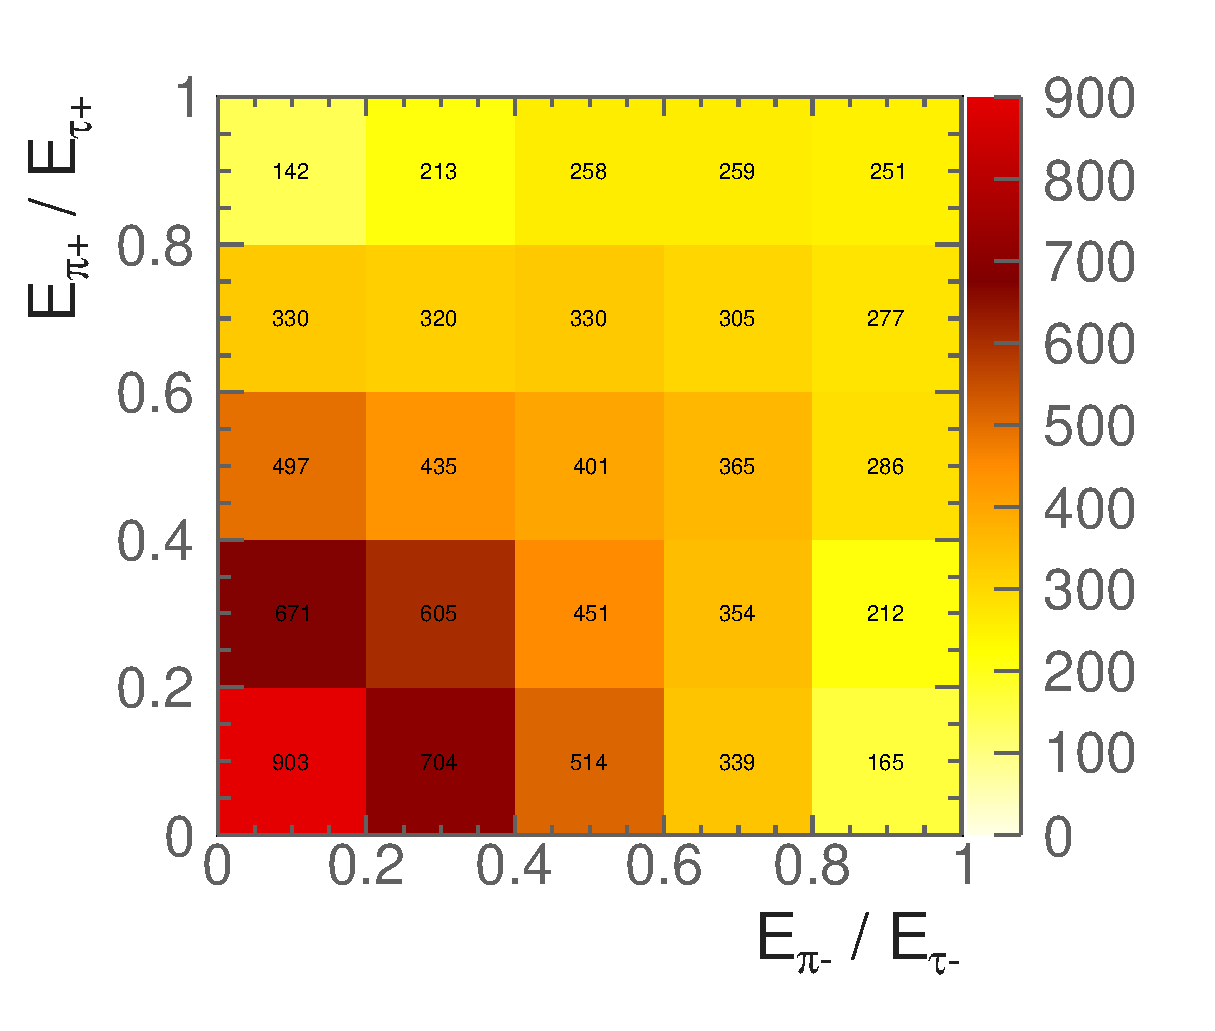
\includegraphics[width=\textwidth]{tau/NoTimeAnalysis/2DNOimproveKE}
  \caption{}
  \label{fig:TauMini2DNOimproveKE}
\end{subfigure}
\begin{subfigure}[b]{0.45\textwidth}
  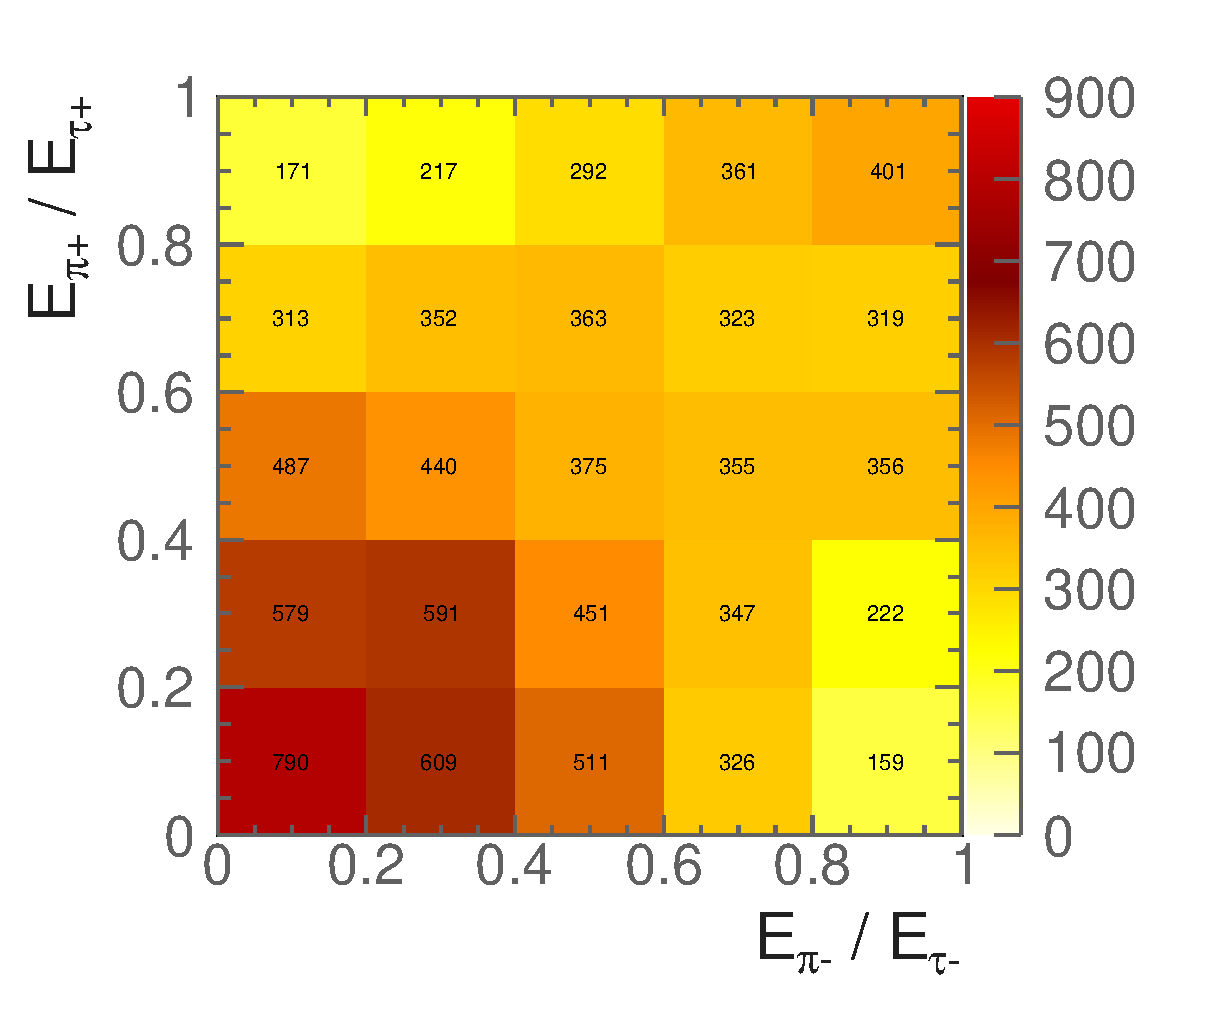
\includegraphics[width=\textwidth]{tau/NoTimeAnalysis/2DimproveKE}
  \caption{}
  \label{fig:TauMini2DimproveKE}
\end{subfigure}
\caption
{Two-dimensional distributions of $E_{\Ppiplus}/E_{\APtauon}$ as a function of $E_{\Ppiminus}/E_{\Ptauon}$ from \ZToTauTau decay where both \tauToPionBoth, with: a)   the  unimproved four-momentum of   \ZForTauTau; and b) the   improved four-momentum of   \ZForTauTau.  \tauToPionBoth decay mode is determined using the truth information. True Monte Carlo tau decay particles are used to generate distributions in figures.}
\label{fig:TauMini2DimproveKEAll}
\end{figure}



\begin{comment}



\begin{equation}
p'^{\mu}_{\ZToTauTau} = p^{\mu}_{\ZToTauTau} \times \frac{\frac{1}{2}\sqrtS}{E_{\ZToTauTau}},
\end{equation}
where $E_{\ZToTauTau}$ is the energy competent of the four-vector $p^{\mu}_{\ZToTauTau}$. The $p'^{\mu}_{\ZToTauTau}$ is the final four-momentum of  the \ZToqq system used to boost tau candidates into the \PZ rest frame.


\begin{equation}
p^{\mu}_{\ZForTauTau} =
  \begin{pmatrix}
    \sqrtS\\   \sqrtS\times\sin\parenths{\theta_{beam}}\\  0   \\       0 \\
  \end{pmatrix}
  - p^{\mu}_{\ZToqq},
\end{equation}


To determine the



Because the energy of the taus can be obtained in the \ZToTauTau rest frame, and events were generated in the \PZ rest frame in the tau decay mode classification study, the tau decay products were boosted into the \PZ rest frame.

In \eeZZQQ events, the four-momentum of the \ZToqq system is measured directly from the particles that are not the tau candidates. The four-momentum of the \ZToTauTau system is obtained by recoiling the four-momentum of the \ZToqq system against the centre-of-mass energy:
\begin{equation}
p^{\mu}_{\ZToTauTau} =
  \begin{pmatrix}
    \sqrtS\\   \sqrtS\times\sin\parenths{\theta_{beam}}\\  0   \\       0 \\
  \end{pmatrix}
  - p^{\mu}_{\ZToqq},
\end{equation}
where $\theta_{beam}$ is the beam crossing angle of  14\,mrad; \sqrtS is the centre-of-mass energy; $p^{\mu}_{\ZToqq}$ is the four-momentum of the \ZToqq system.


\end{comment}
\begin{comment}
 and other variables are defined in the same way as in the previous equation. The vector $p^{\mu}_{\Ptau\Ptau,correct} $ is then treated as the four-momentum vector of \PZ boson, where \ZToTauTau. Tau decay products are boosted to the \PZ decay rest frame accordingly. The calculation of the variables used in the MVA classifier are then performed in the \ZToTauTau decay rest frame.

 $p^{\mu}_{\Ptau\Ptau}$ is the four-momentum vector of the \PZ, where \ZToTauTau; and  index $i$ is summed over all non-tau-decay-product \PFOs. Extra kinematic constraint fixes the energy of the \PZ boson to be a half of \sqrtS:


To use the tau decay mode classifier, it is necessary to know the tau lepton energy to calculate the variables used in the classifier. For the channel \HepProcess{\PZ \to \APtauon \Ptauon}, the  energy of the tau lepton can be obtained in \ZToTauTau decay rest frame, which is half of the \PZ boson energy in the \ZToTauTau rest frame. Hence the tau decay products need to be boosted to the \ZToTauTau decay rest frame for the calculation of the variables used in the MVA classification.

%The boosting requires the \fourMomentum of the \PZ.

The boosting of the tau decay product requires the \fourMomentum of the Z boson, where \ZToTauTau, which is calculated from the recoil momenta of non tau-decay-products:
\begin{equation}
p^{\mu}_{\Ptau\Ptau} =
  \begin{pmatrix}
    \sqrtS\\   \sqrtS\times\sin\parenths{\theta_{beam}}\\  0   \\       0 \\
  \end{pmatrix}
  - \sum_{i}^{non-\Ptau}p^{\mu}_{i},
\end{equation}
where $\theta_{beam}$ is the beam crossing angle; \sqrtS is the centre-of-mass energy; $p^{\mu}_{i}$ is the four-momentum vector of the particle $i$; $p^{\mu}_{\Ptau\Ptau}$ is the four-momentum vector of the \PZ, where \ZToTauTau; and  index $i$ is summed over all non-tau-decay-product \PFOs. Extra kinematic constraint fixes the energy of the \PZ boson to be a half of \sqrtS:
\begin{equation}
p^{\mu}_{\Ptau\Ptau,correct} = p^{\mu}_{\Ptau\Ptau} \times \frac{\frac{1}{2}\sqrtS}{E_{\Ptau\Ptau}},
\end{equation}
where $E_{\Ptau\Ptau}$ is the energy of the vector $p^{\mu}_{\Ptau\Ptau}$  and other variables are defined in the same way as in the previous equation. The vector $p^{\mu}_{\Ptau\Ptau,correct} $ is then treated as the four-momentum vector of \PZ boson, where \ZToTauTau. Tau decay products are boosted to the \PZ decay rest frame accordingly. The calculation of the variables used in the MVA classifier are then performed in the \ZToTauTau decay rest frame.
\end{comment}

\section{Tau decay mode classification}

The tau decay mode classifier developed in \Chapter{chap:Tau} can now be used to select the \tauToPionBoth decay mode. In the classifier, variables regarding EM shower profiles, calorimeter hit information, and track information are not used (the last three rows in \Table{tab:tauVaraibles}) as the information was not available in the outputs of the standard version of \pandora.

% The selection of the \tauToPionBoth decay mode also demands that there is at least one charged pion in the \tauToPionBoth decays.

\begin{comment}

Variables used in  the classifier are a subset of the ones listed in \Table{tab:tauVaraibles}. Variables regarding EM shower profiles, calorimeter hit information, and track information are not used (the last three rows in \Table{tab:tauVaraibles}) as the information was not available in the outputs of the standard version of \pandora used in this analysis.

Variables used in  the MVA classifier are a subset of the ones listed in \Table{tab:tauVaraibles}. Variables regarding EM shower profiles, calorimeter hit information, and track information are not used (the last three rows in \Table{tab:tauVaraibles}) as the information was not available in the outputs of the standard version of \pandora used in this analysis.

%Also for the computational reason, it was not feasible to use these variables for the MVA. \Pep and \Ppiplus separation could be improved if these extra variables are included.


\subsection{Multivariate analysis}

The training  the multivariate classifier follows the procedure in  \Section{sec:tauMVA}. The same classifier with the same parameters as in the previous tau decay mode classification  is used.   In the tau decay mode classifier applying stage, \tauToPion decay mode is selected with an additional criteria that there is at least one charged pion among the tau decay products.
\end{comment}
%\subsection{Result}

\section{Tau pair polarisation correlations}
\label{sec:TauMiniCorr}

\FIGURE{fig:TauSpin1D} shows the one-dimensional distributions of $E_{\Ppiplus} / E_{\APtauon}$ and $E_{\Ppiminus} / E_{\Ptauon}$, using generated \eeZZQQ events. Both taus decay by \tauToPionBoth. $E_{\Ptaupm}$ is half of the energy of \ZForTauTau in \ZForTauTau rest frame.  At the generator level, the shape of the distribution decreases gradually with the increasing $E_{\Ppipm}/E_{\Ptaupm}$. The decreasing shape is largely preserved in the full detector simulation. In the full detector simulation, events with  $E_{\Ppipm}/E_{\Ptaupm}$ close to 0, which fall in the first bin in the figures, are not reconstructed correctly. When the energies of the tau are mostly carried away by the neutrinos, it is difficult to identify low-energy charged pions as tau decay products.


%The energy fractions of the tau decay product to the tau lepton ($E_{\Ppiplus} / E_{\APtauon}$ and $E_{\Ppiminus} / E_{\Ptauon}$) are the appropriate kinematic variables to study the tau pair polarisation correlation, motivated in \Section{sec:theoryTauPair}.

\begin{figure}[htbp]
\centering % \begin{center}/\end{center} takes some additional vertical space
\begin{subfigure}[b]{0.45\textwidth}
  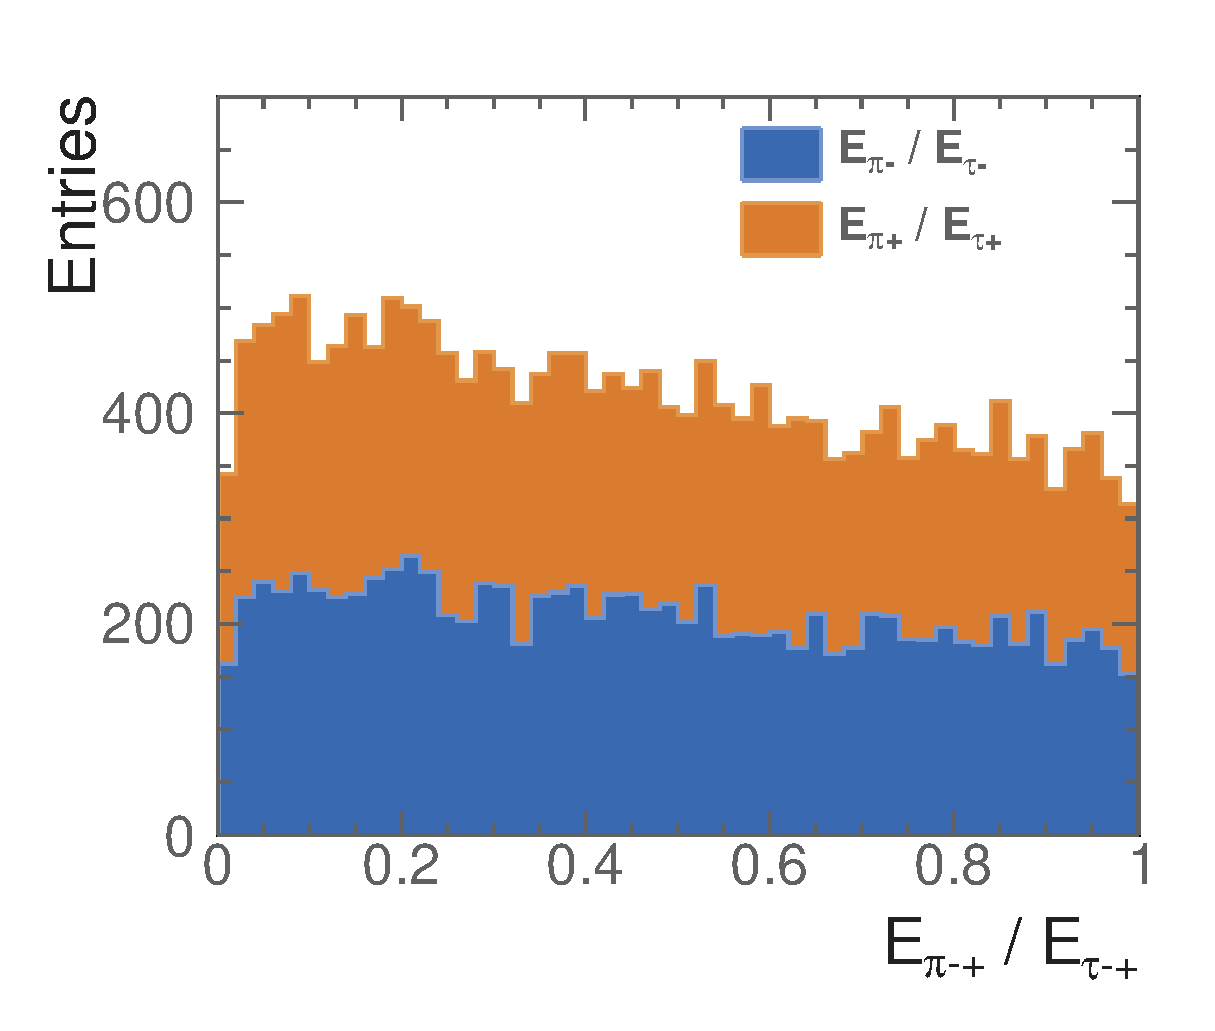
\includegraphics[width=\textwidth]{tau/NoTimeAnalysis/1DMC}
  \caption{}
  \label{fig:TauSpin1DMC}
\end{subfigure}
\begin{subfigure}[b]{0.45\textwidth}
  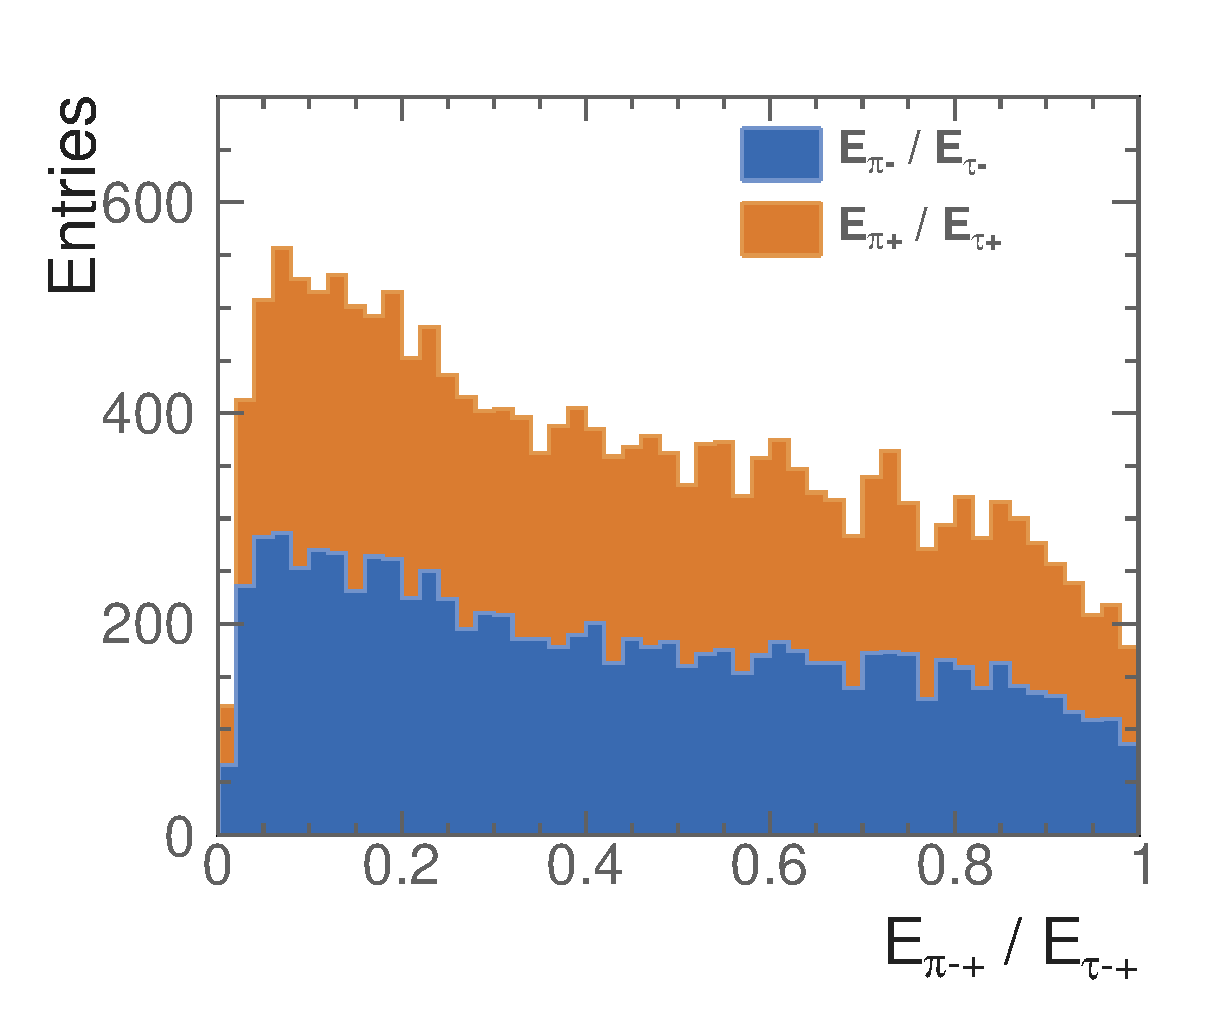
\includegraphics[width=\textwidth]{tau/NoTimeAnalysis/1DrecoNoOverflow}
  \caption{}
  \label{fig:TauSpin1Dreco}
\end{subfigure}
\caption
{Distributions of $E_{\Ppipm}/E_{\Ptaupm}$ from \ZToTauTau decays where both \tauToPionBoth, in \eeZZQQ events for: a) generator-level  Monte Carlo particles, and b) the full detector simulation. The \tauToPionBoth decay mode is selected using: a) the truth information; and b) the tau decay mode classifier.}
\label{fig:TauSpin1D}
\end{figure}



%The energy fractions of the tau decay product to the tau lepton ($E_{\Ppiplus} / E_{\APtauon}$ and $E_{\Ppiminus} / E_{\Ptauon}$) are the appropriate kinematic variables to study the tau pair polarisation correlation, motivated in \Section{sec:theoryTauPair}.


%tau decay product energy fractions, with \eeZZ channel where one \PZ decays to a tau pair and the other \PZ decays hadronically, using both \tauToPion decay mode.

\FIGURE{fig:TauSpin2D} shows the two-dimensional distributions of $E_{\Ppiplus} / E_{\APtauon}$ versus $E_{\Ppiminus} / E_{\Ptauon}$, using generated \eeZZQQ events. Both taus decay by \tauToPionBoth. \FIGURE{fig:TauSpin2DMC} shows the  two-dimensional  tau decay product energy fraction distribution obtained with the generator-level  Monte Carlo particles. \FIGURE{fig:TauSpin2Dreco} shows the distribution using the full detector simulation. A good match between the distributions obtained with  the generator-level  MC particles and the full detector simulation is achieved. Dark regions along the diagonal can be seen in both the distribution for the Monte Carlo particles and the distribution for the full detector simulation. In the \ZToTauTau decays, where both \tauToPionBoth, an energetic \Pgppm is likely to be associated with an energetic \Pgpmp and a low-energy \Pgppm is  likely to be associated with a low-energy \Pgpmp. Comparing the two figures, some events in the top right quadrant, corresponding to  both \Ppipm being energetic, are not reconstructed correctly in the full detector simulation, due to the failure of identifying the correct tau decay products.


\begin{figure}[htbp]
\centering % \begin{center}/\end{center} takes some additional vertical space
\begin{subfigure}[b]{0.7\textwidth}
  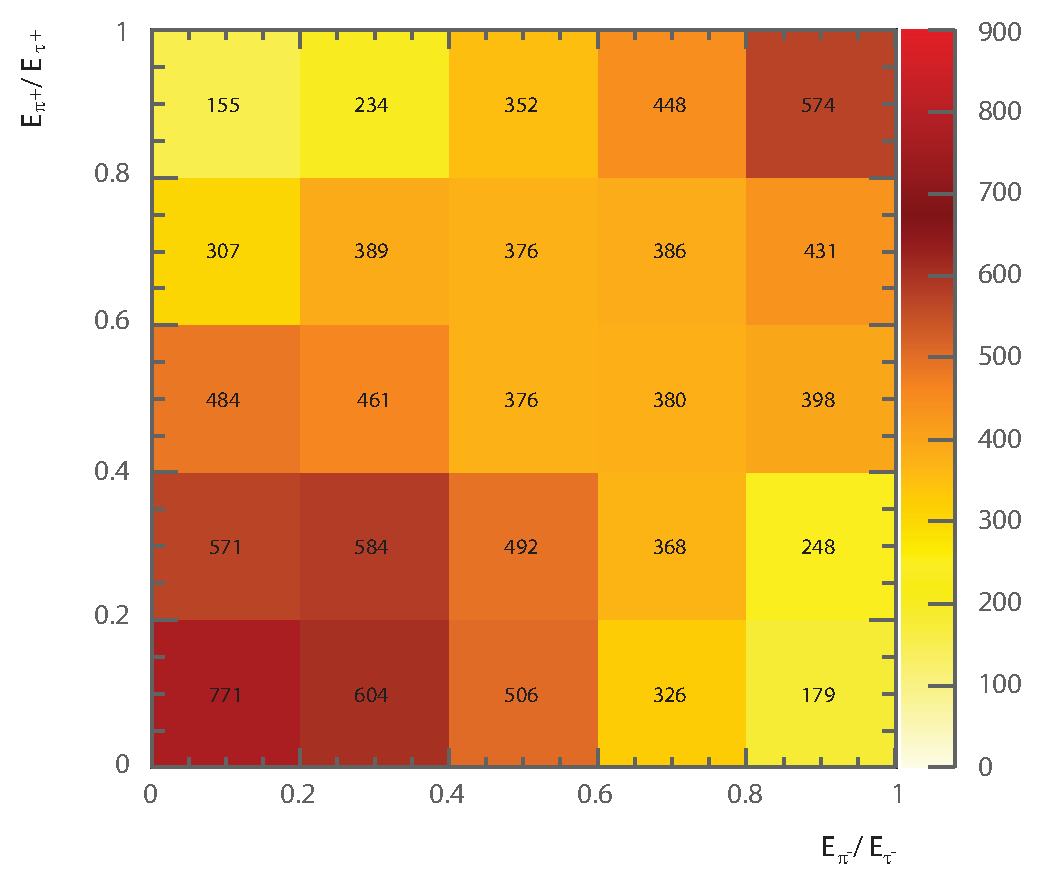
\includegraphics[width=\textwidth]{tau/NoTimeAnalysis/2DMC2}
  \caption{Generator-level  Monte Carlo particles}
  \label{fig:TauSpin2DMC}
\end{subfigure}
\begin{subfigure}[b]{0.7\textwidth}
  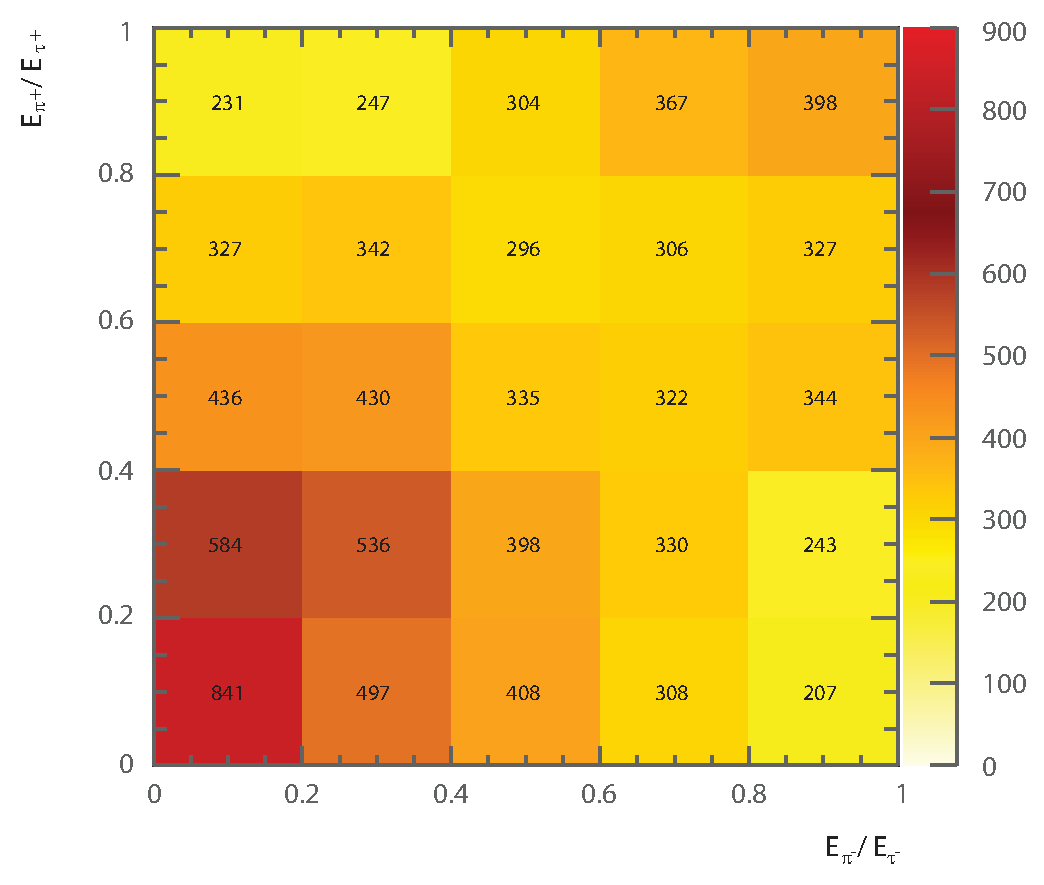
\includegraphics[width=\textwidth]{tau/NoTimeAnalysis/2Dreco2}
  \caption{Full detector simulation}
  \label{fig:TauSpin2Dreco}
\end{subfigure}
\caption
{Two-dimensional distributions of $E_{\Ppiplus}/E_{\APtauon}$ as a function of $E_{\Ppiminus}/E_{\Ptauon}$ from \ZToTauTau decays where both \tauToPionBoth, in \eeZZQQ events for: a) generator-level  Monte Carlo particles; and b) the full detector simulation. The \tauToPionBoth decay mode is selected using: a) the truth information; and b) the tau decay mode classifier.}
\label{fig:TauSpin2D}
\end{figure}

\section{Summary}
This is a proof-of-principle demonstration that the generator-level pion energy fraction correlation can be reconstructed at the analysis level. The analysis contains several important steps: tau identification; kinematic reconstruction of the energies of the taus; the classification of the  \tauToPionBoth decay mode; and the reconstruction of the tau pair polarisation correlations discussed in \Section{sec:theoryTauPair}.

%the incorrect finding of the tau pair decay products  in \Section{sec:tauHZfindTau}.


% This trend is shown in both the distribution produced with the Monte Carlo particles and with the full detector simulation

%This proof-of-principle analysis shows the tau polarisation correlations, using the \eeZZ channel where one \PZ decays hadronically and the other \PZ decays to a tau pair and subsequently both \tauToPion,  is possible to be observed with the \ILD detector model at \rootSGeV{350}. With a similar study of the \eeHZ channel where \PH decays hadronically and \PZ decays to a tau pair and both \tauToPion,  the  tau pair decay products energy distribution can be used to statistically identify if the parent boson is a Higgs boson or a \PZ boson.

%, and to identify Higgs boson in an experiment that observes the breaking of the lepton universality by favouring tau pair events.


%If the tau pair decay from Higgs boson is observed, the decay can be recognised in the \tauToPion mode as a high-energy \Pgppm with a low-energy \Pgpmp. Hence, the tau decay product energy distribution can be a clean signature for \HiggsToTauTau.

%\FIGURE{fig:theoryTauPairCorrelation} shows the resulting two-dimensional distributions of  $\overline{z} = \frac{E_{\Ppiplus}}{E_{\APtauon}}$ versus  $z = \frac{E_{\Ppiminus}}{E_{\Ptauon}}$ for \ZToTauTau and \HiggsToTauTau channels, where both tau leptons decay via \tauToPion. The difference of the tau pair polarisation correlation between \PZ and \PHiggs  is clear. The energy distribution of the charged pion from \ZToTauTau has the form of $\overline{z}  \sim z$, whilst the distribution from  \HiggsToTauTau has the form of $\overline{z}  \sim (1-z)$. Therefore, in \ZToTauTau process, a high-energy \Pgppm  is likely to be associated with a high-energy \Pgpmp. In \HiggsToTauTau process, the opposite is favoured. If the tau pair decay from Higgs boson is observed, the decay can be recognised in the \tauToPion mode as a high-energy \Pgppm with a low-energy \Pgpmp. Hence, the tau decay product energy distribution can be a clean signature for \HiggsToTauTau.



\begin{comment}
\begin{figure}[htbp]
\centering % \begin{center}/\end{center} takes some additional vertical space
\begin{subfigure}[b]{0.45\textwidth}
  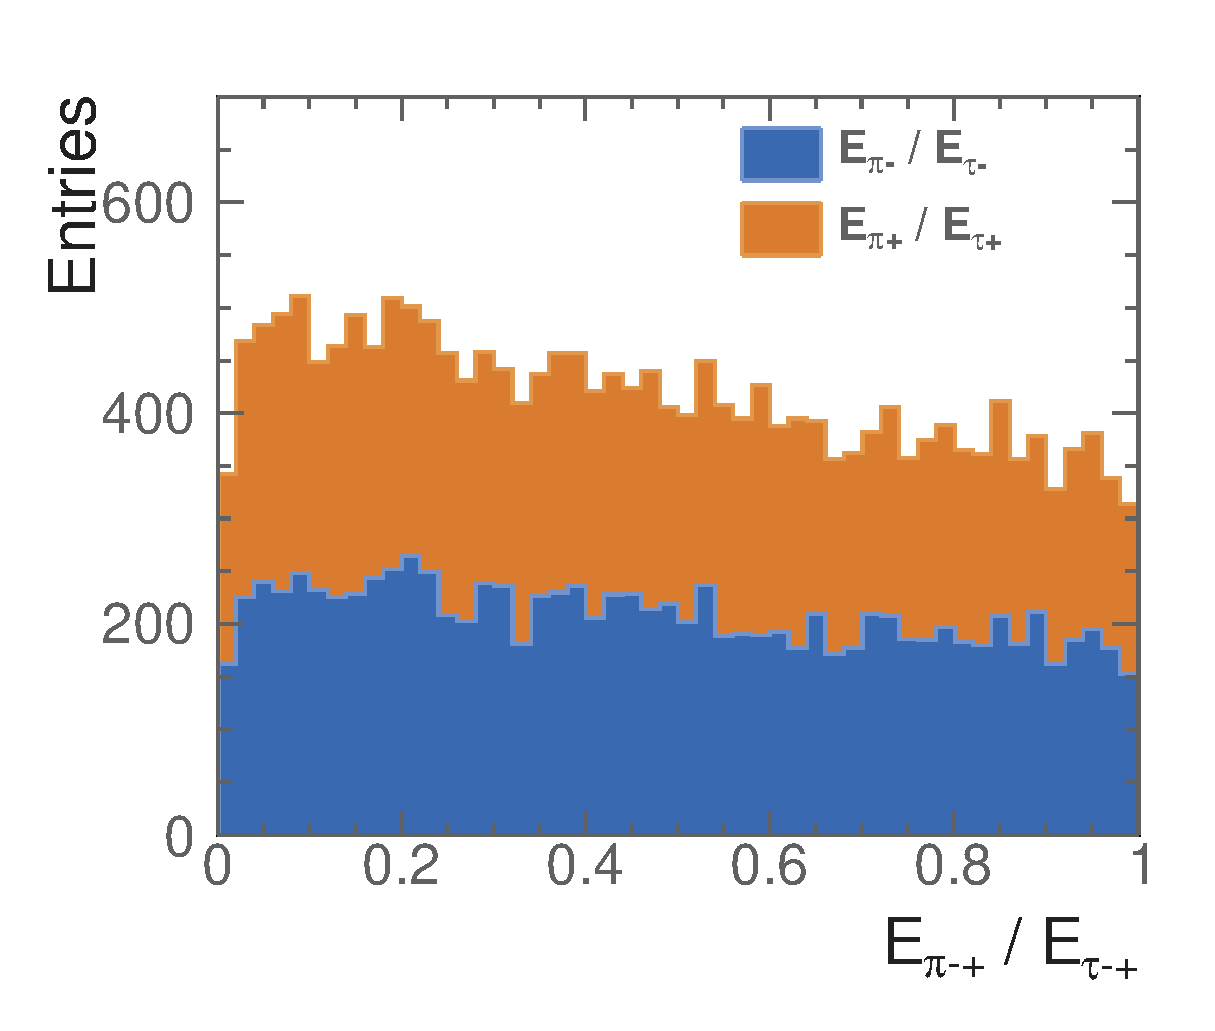
\includegraphics[width=\textwidth]{tau/NoTimeAnalysis/1DMC}
  \caption{Truth info.}
  \label{fig:TauSpin1DMC}
\end{subfigure}
\begin{subfigure}[b]{0.45\textwidth}
  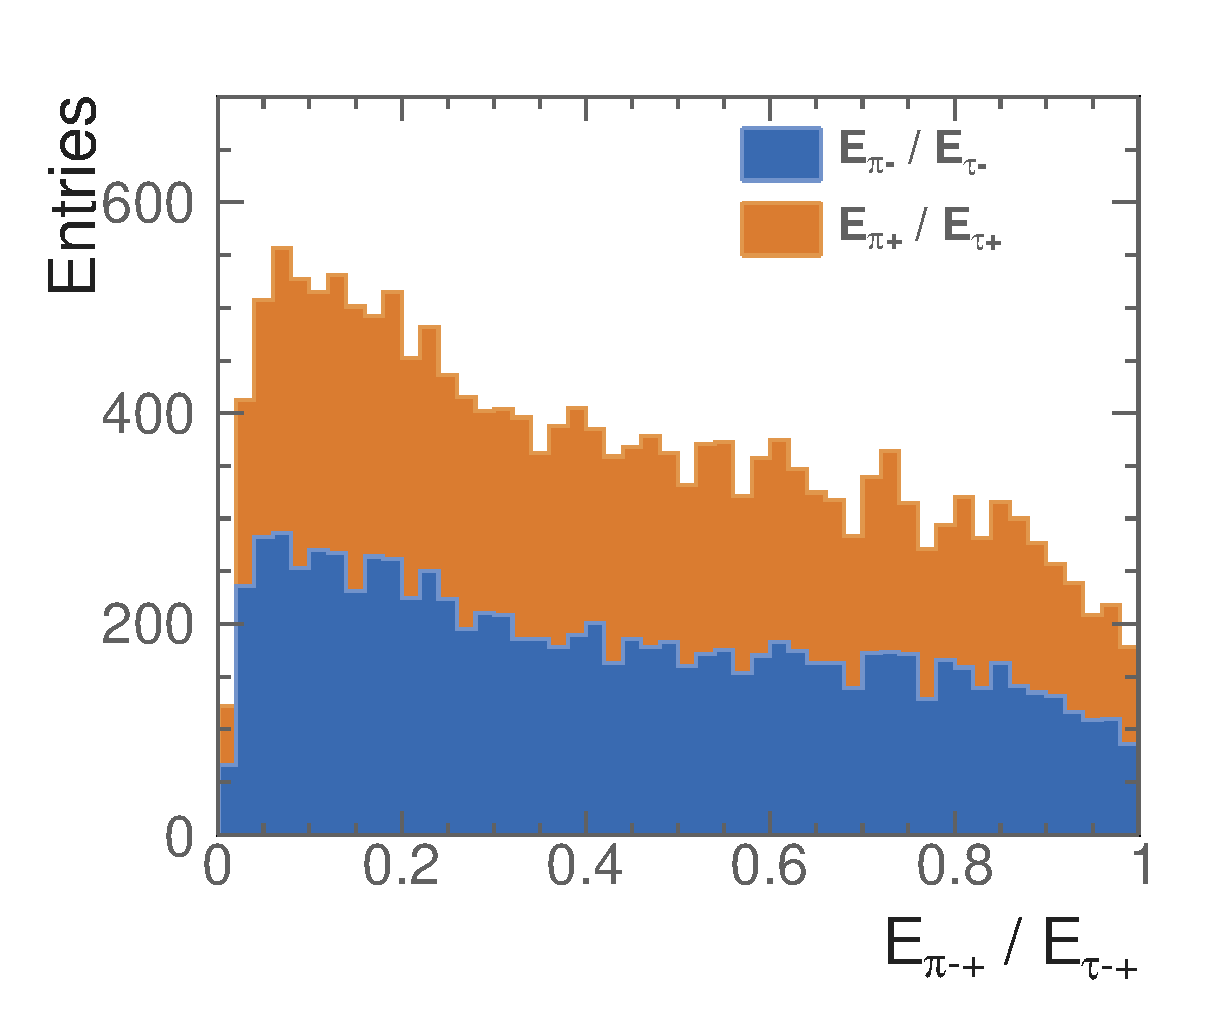
\includegraphics[width=\textwidth]{tau/NoTimeAnalysis/1DrecoNoOverflow}
  \caption{Reconstructed}
  \label{fig:TauSpin1Dreco}
\end{subfigure}
\caption[One-dimensional plot of spin correlations of the tau lepton pair from \PZ decay, using \decayPionShort decay mode.]
{One-dimensional plot of spin correlations of the tau lepton pair from \PZ decay, using \decayPionShort decay mode.}
\label{fig:TauSpin1D}
\end{figure}

\end{comment} 